%%%%%%%%%%%%%%%%%%%%%%%%%%%%%%%%%%%%%%%%%%%%%%%%%%%%%%%%%%%%%%%%%%%%%%%%%%%%%%%%
%2345678901234567890123456789012345678901234567890123456789012345678901234567890
%        1         2         3         4         5         6         7         8

\documentclass[letterpaper, 10 pt, conference]{ieeeconf}  % Comment this line out if you need a4paper

%\documentclass[a4paper, 10pt, conference]{ieeeconf}      % Use this line for a4 paper

%\IEEEoverridecommandlockouts                              % This command is only needed if 
                                                          % you want to use the \thanks command

\overrideIEEEmargins                                      % Needed to meet printer requirements.

% See the \addtolength command later in the file to balance the column lengths
% on the last page of the document

% The following packages can be found on http:\\www.ctan.org
%\usepackage{graphics} % for pdf, bitmapped graphics files
%\usepackage{epsfig} % for postscript graphics files
%\usepackage{mathptmx} % assumes new font selection scheme installed
%\usepackage{times} % assumes new font selection scheme installed
%\usepackage{amsmath} % assumes amsmath package installed
%\usepackage{amssymb}  % assumes amsmath package installed
\usepackage{graphicx} % for pdf, bitmapped graphics files
\usepackage{float}
\usepackage{caption}
\usepackage{subcaption}
%\usepackage{algorithm,algpseudocode}

%\usepackage{epsfig} % for postscript graphics files
%\usepackage{mathptmx} % assumes new font selection scheme installed
%\usepackage{times} % assumes new font selection scheme installed
\usepackage{amsmath} % assumes amsmath package installed
%\usepackage{amssymb}  % assumes amsmath package installed
\usepackage{enumerate}

\title{Project Report:\\\LARGE \bf
Stereo Matching using Graphcut-based Optimization}

\author{Seyed Abbas Sadat\\
Simon Fraser University\\
sas21@sfu.ca% <-this % stops a space
}


\begin{document}



\maketitle
\thispagestyle{empty}
\pagestyle{empty}

%%%%%%%%%%%%%%%%%%%%%%%%%%%%%%%%%%%%%%%%%%%%%%%%%%%%%%%%%%%%%%%%%%%%%%%%%%%%%%%%

\section{INTRODUCTION}

\begin{figure*}[t]
        \centering
        \begin{subfigure}[b]{0.3\textwidth}
                \centering
                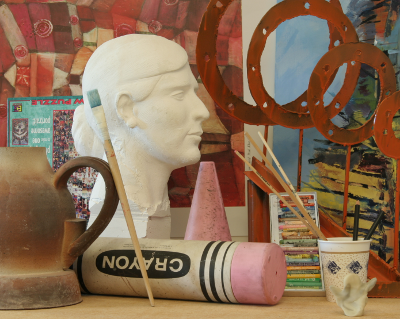
\includegraphics[width=\textwidth]{imgs/l4.png}
                \caption{"Art" Color image}
                \label{fig:trees}
        \end{subfigure}%
                ~ %add desired spacing between images, e. g. ~, \quad, \qquad etc.
          %(or a blank line to force the subfigure onto a new line)
        \begin{subfigure}[b]{0.3\textwidth}
                \centering
                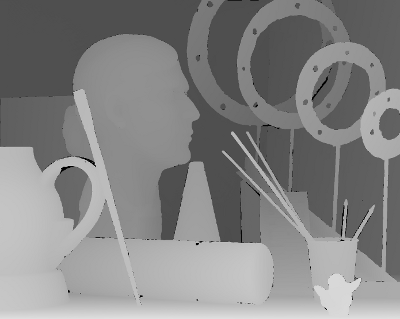
\includegraphics[width=\textwidth]{imgs/disp4.png}
                \caption{Ground Truth}
                \label{fig:farm}
        \end{subfigure}
                ~ %add desired spacing between images, e. g. ~, \quad, \qquad etc.
          %(or a blank line to force the subfigure onto a new line)
        \begin{subfigure}[b]{0.3\textwidth}
                \centering
                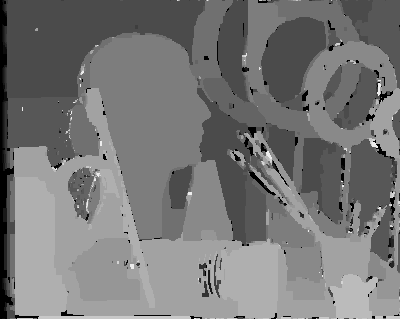
\includegraphics[width=\textwidth]{imgs/l4disparity-expansion.png}
                \caption{$\alpha$-expansion}
                \label{fig:farm}
        \end{subfigure}
                ~ %add desired spacing between images, e. g. ~, \quad, \qquad etc.
          %(or a blank line to force the subfigure onto a new line)
        \begin{subfigure}[b]{0.3\textwidth}
                \centering
                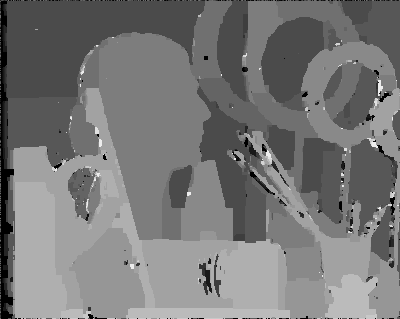
\includegraphics[width=\textwidth]{imgs/l4disparity-swap.png}
                \caption{$\alpha\beta$-swap}
                \label{fig:farm}
        \end{subfigure}
                        ~ %add desired spacing between images, e. g. ~, \quad, \qquad etc.
          %(or a blank line to force the subfigure onto a new line)
        \begin{subfigure}[b]{0.3\textwidth}
                \centering
                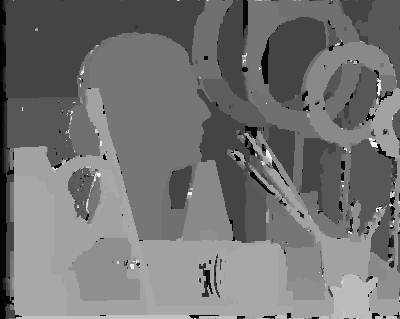
\includegraphics[width=\textwidth]{imgs/l4disparity-expansion-sub.png}
                \caption{$\alpha$-expansion - subpixel accuracy}
                \label{fig:farm}
        \end{subfigure}
                ~ %add desired spacing between images, e. g. ~, \quad, \qquad etc.
          %(or a blank line to force the subfigure onto a new line)
        \begin{subfigure}[b]{0.3\textwidth}
                \centering
                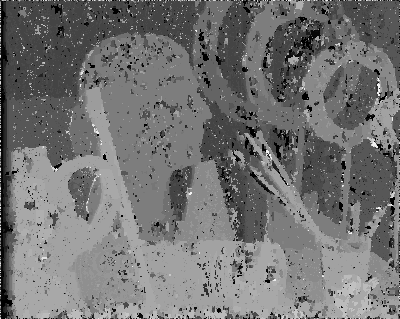
\includegraphics[width=\textwidth]{imgs/l4disparity-swap-sub.png}
                \caption{$\alpha\beta$-swap - subpixel accuracy}
                \label{fig:farm}
        \end{subfigure}
        \caption{Disparity image for the "Art" dataset using the both $\alpha\beta$-swap and $\alpha$-expansion with pixel and subpixel accuracies.}
        \label{fig:realmaps}
\end{figure*}

\begin{figure*}[t]
        \centering
        \begin{subfigure}[b]{0.3\textwidth}
                \centering
                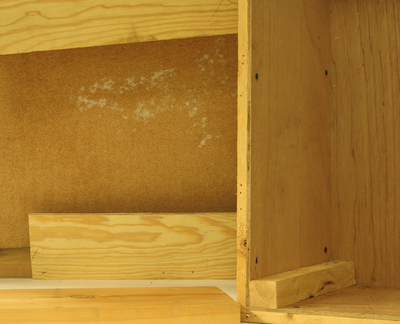
\includegraphics[width=\textwidth]{imgs/l2.png}
                \caption{"Wood1" Color image}
                \label{fig:trees}
        \end{subfigure}%
                ~ %add desired spacing between images, e. g. ~, \quad, \qquad etc.
          %(or a blank line to force the subfigure onto a new line)
        \begin{subfigure}[b]{0.3\textwidth}
                \centering
                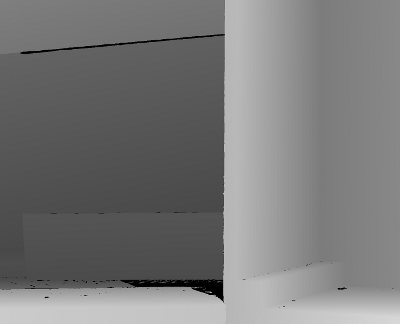
\includegraphics[width=\textwidth]{imgs/disp2.png}
                \caption{Ground Truth}
                \label{fig:farm}
        \end{subfigure}
                ~ %add desired spacing between images, e. g. ~, \quad, \qquad etc.
          %(or a blank line to force the subfigure onto a new line)
        \begin{subfigure}[b]{0.3\textwidth}
                \centering
                
\includegraphics[width=\textwidth]{imgs/l2disparity-expansion.png}
                \caption{$\alpha$-expansion}
                \label{fig:farm}
        \end{subfigure}
                ~ %add desired spacing between images, e. g. ~, \quad, \qquad etc.
          %(or a blank line to force the subfigure onto a new line)
        \begin{subfigure}[b]{0.3\textwidth}
                \centering
                
\includegraphics[width=\textwidth]{imgs/l2disparity-swap.png}
                \caption{$\alpha\beta$-swap}
                \label{fig:farm}
        \end{subfigure}
                        ~ %add desired spacing between images, e. g. ~, \quad, \qquad etc.
          %(or a blank line to force the subfigure onto a new line)
        \begin{subfigure}[b]{0.3\textwidth}
                \centering
                
\includegraphics[width=\textwidth]{imgs/l2disparity-expansion-sub.png}
                \caption{$\alpha$-expansion - subpixel accuracy}
                \label{fig:farm}
        \end{subfigure}
                ~ %add desired spacing between images, e. g. ~, \quad, \qquad etc.
          %(or a blank line to force the subfigure onto a new line)
        \begin{subfigure}[b]{0.3\textwidth}
                \centering
                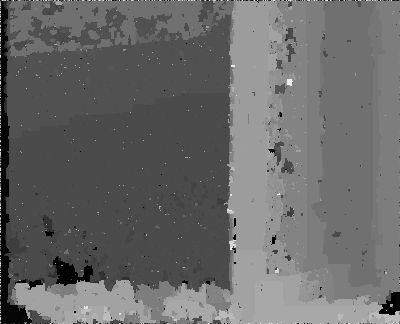
\includegraphics[width=\textwidth]{imgs/l2disparity-swap-sub.png}
                \caption{$\alpha\beta$-swap - subpixel accuracy}
                \label{fig:farm}
        \end{subfigure}
        \caption{Disparity image for the "Wood1" dataset using the both $\alpha\beta$-swap and $\alpha$-expansion with pixel and subpixel accuracies.}
        \label{fig:realmaps}
\end{figure*}

In this project we developed a stereo matching system based on graph-cut optimization framework \cite{boykov2001fast}. In stereo matching problem, 2 images taken from 2 cameras that are on the same horizontal line are to be matched pixel by pixel. Therefore, for each pixel on the left image, we should find its corresponding pixel on the right image. According to the assumptions, we know that if $(i,j)$ is the coordinate of the pixel in the left image, the coordinate of the corresponding pixel in the right image will be $(i,j-d)$. The unknown variable $d$ is called disparity and is defined in the image space. Disparity is inversely proportional to the depth of the pixel, i.e., the higher the disparity the closer the object. The disparity is not always observable using only 2 images because part of the scene can be occluded in either of the left or right images and hence no matched pixel can be found.

The stereo matching problem is formulated as: given a left and right image, find the most probable disparity image. This $maximum a posteriori$ problem is often solved by finding a disparity image that minimizes some energy function. The energy function includes some terms that promote data fidelity (data terms) as well as other terms that support prior assumptions about the solution, e.g., smoothness (smoothness term). These energy functions are non-convex and finding a global optimum it very difficult. Instead, approaches that result in approximation solutions are preferred. One way to reach a local optimum in the minimization is to perform gradient descent. Graph-cuts offer a framework that enables us to generate a movement (step) of current solution that is steepest in terms of minimizing the energy function. By generating and performing these steps iteratively, we reach a local optimum. 

In section \ref{graphcut} we briefly explain how to generate gradient descent moves for a general pixel labelling problem.

\section{Graphcut-based Optimization}
\label{graphcut}
The energy function that we use for stereo matching has the following form:
\begin{figure}[h]
                \centering
                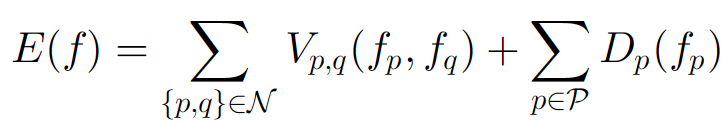
\includegraphics[width=0.35\textwidth]{imgs/energy.png}
                \label{fig:farm}
\end{figure}

\section{Stereo Matching}
\section{Experiments and Results}
\bibliographystyle{ieeetr} 
\bibliography{refs}


\end{document}
